\section{Вписанные углы}

\paragraph{Вписанный угол.}\label{1938/123}
Угол, образованный двумя хордами, исходящими из одной точки окружности, называется \rindex{вписанный угол}\textbf{вписанным} углом.
Таков, например, угол $ABC$ (рис.~\ref{1938/ris-137}).

О вписанном угле принято говорить, что он опирается на дугу, заключённую между его сторонами.
Так, угол $ABC$ \rindex{опирается на дугу}\textbf{опирается} на дугу $AC$.

\paragraph{}\label{1938/124} 
\so{Теорема}.
\textbf{\emph{Вписанный угол измеряется половиной дуги, на которую он опирается.}}
Эту теорему надо понимать так:
вписанный угол содержит в себе столько угловых градусов, минут и секунд, сколько дуговых градусов, минут и секунд заключается в половине дуги, на которую он опирается.

\begin{figure}[h]
\begin{minipage}{.32\textwidth}
\centering
\includegraphics{mppics/ris-137}
\end{minipage}
\hfill
\begin{minipage}{.32\textwidth}
\centering
\includegraphics{mppics/ris-138}
\end{minipage}
\hfill
\begin{minipage}{.32\textwidth}
\centering
\includegraphics{mppics/ris-139}
\end{minipage}

\medskip

\begin{minipage}{.32\textwidth}
\centering
\caption{}\label{1938/ris-137}
\end{minipage}
\hfill
\begin{minipage}{.32\textwidth}
\centering
\caption{}\label{1938/ris-138}
\end{minipage}
\hfill
\begin{minipage}{.32\textwidth}
\centering
\caption{}\label{1938/ris-139}
\end{minipage}
\vskip-4mm
\end{figure}

При доказательстве теоремы рассмотрим особо три случая:

1) Центр $O$ (рис.~\ref{1938/ris-137}) лежит на стороне вписанного угла $ABC$.
Проведя радиус $AO$, мы получим $\angle AOB$, в котором $OA \z= OB$ (как радиусы), и, следовательно, $\angle ABO\z=\angle BAO$.
По отношению к этому треугольнику угол $AOC$ есть внешний, поэтому он равен сумме углов $ABO$ и $BAO$ и, значит, равен двум углам $ABO$;
поэтому угол $ABO$ равен половине центрального угла $AOC$.
Но угол $AOC$ измеряется дугой $AC$, то есть
он содержит в себе столько угловых градусов, минут и секунд, сколько дуговых градусов, минут и секунд содержится в дуге $AC$;
следовательно, вписанный угол $ABC$ измеряется половиной дуги $AC$.

2) Центр $O$ лежит между сторонами вписанного угла $ABC$ (рис.~\ref{1938/ris-138}).

Проведя диаметр $BD$, мы разделим угол $ABC$ на два угла, из которых, по доказанному, один измеряется половиной дуги $AD$, а другой — половиной дуги $DC$;
следовательно, угол $ABC$ измеряется суммой
\[\tfrac12{\smallsmile}AD\z+\tfrac12{\smallsmile}DC=\tfrac12({\smallsmile}AD\z+{\smallsmile}DC)=\tfrac12{\smallsmile}AC.\]


3) Центр $O$ лежит вне вписанного угла $ABC$ (рис.~\ref{1938/ris-139}).
Проведя диаметр $BD$, мы будем иметь:
\[\angle ABC=\angle ABD-\angle CBD.\]

Но углы $ABD$ и $CBD$ измеряются, по доказанному, половинами дуг $AD$ и $CD$;
следовательно, угол $ABC$ измеряется разностью
\[\tfrac12{\smallsmile}AD-\tfrac12{\smallsmile}CD=\tfrac12({\smallsmile}AD-{\smallsmile}CD)=\tfrac12{\smallsmile}AC.\]

\begin{figure}[h]
\begin{minipage}{.48\textwidth}
\centering
\includegraphics{mppics/ris-140}
\end{minipage}
\hfill
\begin{minipage}{.48\textwidth}
\centering
\includegraphics{mppics/ris-141}
\end{minipage}

\medskip

\begin{minipage}{.48\textwidth}
\centering
\caption{}\label{1938/ris-140}
\end{minipage}
\hfill
\begin{minipage}{.48\textwidth}
\centering
\caption{}\label{1938/ris-141}
\end{minipage}
\vskip-4mm
\end{figure}

\paragraph{}\label{1938/125}
\so{Следствия}. 
1) \emph{Все вписанные углы, опирающиеся на одну и ту же дугу, равны между собой} (рис.~\ref{1938/ris-140}), потому что каждый из них измеряется половиной одной и той же дуги.
Если величину одного из таких углов обозначим $\alpha$, то можно сказать, что сегмент $AmB$, покрытый на чертеже штрихами, \so{вмещает в себя угол}, равный $\alpha$. 

2) \emph{Всякий вписанный угол, опирающийся на диаметр, есть прямой} (рис.~\ref{1938/ris-141}), потому что каждый такой угол измеряется половиной полуокружности и, следовательно, содержит $90\degree$.



\paragraph{}\label{1938/126}
\so{Задача}.
\emph{Построить прямоугольный треугольник по гипотенузе $a$ и катету $b$} (рис.~\ref{1938/ris-142}).


На какой-нибудь прямой $MN$ отложим $AB=a$, на $AB$ опишем полуокружность.
Затем проводим дугу радиусом, равным $b$, с центром в точке $A$ (или $B$).

Точку пересечения $C$ полуокружности и дуги соединим с концами диаметра $AB$.
Треугольник $ABC$ будет искомый, так как угол $C$ — прямой, $a$ является гипотенузой, а $b$ — катетом.

\begin{figure}[h!]
\begin{minipage}{.48\textwidth}
\centering
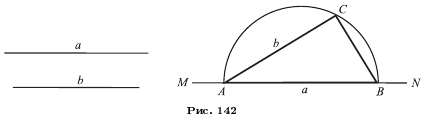
\includegraphics{mppics/ris-142}
\end{minipage}
\hfill
\begin{minipage}{.48\textwidth}
\centering
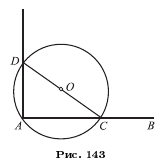
\includegraphics{mppics/ris-143}
\end{minipage}

\medskip

\begin{minipage}{.48\textwidth}
\centering
\caption{}\label{1938/ris-142}
\end{minipage}
\hfill
\begin{minipage}{.48\textwidth}
\centering
\caption{}\label{1938/ris-143}
\end{minipage}
\vskip-4mm
\end{figure}

\paragraph{}\label{1938/127}
\so{Задача}.
\emph{Из конца $A$ \emph{(рис.~\ref{1938/ris-143})} данного луча $AB$, не продолжая его, восстановить к нему перпендикуляр.}

Возьмём вне прямой какую-либо точку $O$ так, чтобы окружность с центром в этой точке и радиусом, равным отрезку $OA$, пересекла луч $AB$ в какой-либо точке $C$.
Через эту точку $C$ проведём диаметр $CD$ и конец его $D$ соединим с $A$.
Прямая $AB$ есть искомый перпендикуляр, потому что угол $A$ прямой, как вписанный и опирающийся на диаметр.


\begin{wrapfigure}{r}{42mm}
\centering
\includegraphics{mppics/ris-145}
\caption{}\label{1938/ris-145}
\end{wrapfigure}

\paragraph{}\label{1938/128}
\mbox{\so{Задача}.}
\emph{Через данную точку провести к касательную к данной окружности.}

Эта задача уже  была решена в §~\ref{1931/115};
мы приведём другое решение случай когда \so{данная точка} ($A$, рис.~\ref{1938/ris-145}) \so{лежит вне окружности} (с центром $O$).

Соединив $A$ с $O$, делим $AO$ пополам в точке $O_1$ и с центром в этой точке радиусом $OO_1$ описываем окружность.
Через точки $B$ и $B_1$, в которых эта окружность пересекается с данной, проводим прямые $AB$ и $AB_1$.
Эти прямые и будут касательными, так как углы $OBA$ и $OB_1A$, как опирающиеся на диаметр, — прямые.




\paragraph{}\label{1938/130}
\so{Теорема}.
1) \textbf{\emph{Угол}} ($ABC$, рис.~\ref{1938/ris-148}), \textbf{\emph{вершина которого лежит внутри круга, измеряется полусуммой двух дуг}} ($AC$ и $DE$), \textbf{\emph{из которых одна заключена между его сторонами, а другая — между продолжениями сторон.}}

2) \textbf{\emph{Угол}} ($ABC$, рис.~\ref{1938/ris-149}), \textbf{\emph{вершина которого лежит вне круга и стороны пересекаются с окружностью, измеряется полуразностью двух дуг}} ($AC$ и $ED$), \textbf{\emph{заключённых между его сторонами.}}

\begin{figure}[h]
\begin{minipage}{.48\textwidth}
\centering
\includegraphics{mppics/ris-148}
\end{minipage}
\hfill
\begin{minipage}{.48\textwidth}
\centering
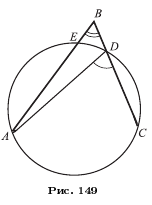
\includegraphics{mppics/ris-149}
\end{minipage}

\medskip

\begin{minipage}{.48\textwidth}
\centering
\caption{}\label{1938/ris-148}
\end{minipage}
\hfill
\begin{minipage}{.48\textwidth}
\centering
\caption{}\label{1938/ris-149}
\end{minipage}
\vskip-4mm
\end{figure}

Проведя хорду $AB$ (на том и на другом чертеже), мы получим $\triangle ABD$, относительно которого рассматриваемый угол $ABC$ служит внешним, когда его вершина лежит внутри круга, и внутренним, когда его вершина лежит вне круга.
Поэтому в первом случае:
\[\angle ABC = \angle ADC+\angle DAE;\]
во втором случае:
\[\angle ABC = \angle ADC-\angle DAE.\]

Но углы $ADC$ и $DAE$, как вписанные, измеряются половинами дуг $AC$ и $BE$, поэтому угол $ABC$ измеряется:
в первом случае суммой
$\tfrac12{\smallsmile}AC+\tfrac12{\smallsmile}DE$, которая равна $\tfrac12({\smallsmile}AC+{\smallsmile}DE)$, а во втором случае разностью $\tfrac12{\smallsmile}AC-\tfrac12{\smallsmile}DE$, которая равна $\tfrac12({\smallsmile}AC-{\smallsmile}DE)$.

\paragraph{}\label{1938/131}
\so{Теорема}.
\textbf{\emph{Угол}} ($ACD$, рис.~\ref{1938/ris-150} и \ref{1938/ris-151}), \textbf{\emph{составленный касательной и хордой, измеряется половиной дуги, заключённой внутри него.}}

\begin{wrapfigure}{o}{30mm}
\centering
\includegraphics{mppics/ris-150}
\caption{}\label{1938/ris-150}
\bigskip
\includegraphics{mppics/ris-151}
\caption{}\label{1938/ris-151}
\end{wrapfigure}

Предположим сначала, что хорда $CD$ проходит через центр $O$, то есть что эта хорда есть диаметр (рис.~\ref{1938/ris-150}).
Тогда угол $ACD$ — прямой и,
следовательно, равен $90\degree$.
Но и половина дуги $CmD$ также равна $90\degree$, так как целая дуга $CmD$, составляя полуокружность, содержит $180\degree$.
Значит, теорема справедлива в этом частном случае.

Рассмотрим общий случай (рис.~\ref{1938/ris-151}), когда хорда $CD$ не проходит через центр.
Проведя диаметр $CE$, мы будем иметь:
\[\angle ACD = \angle ACE - \angle DCE.\]

Угол $ACE$, как составленный касательной и диаметром, измеряется, по доказанному, половиной дуги $CDE$;
угол $DCE$, как вписанный, измеряется половиной дуги $DE$;
следовательно, угол $ACD$ измеряется разностью $\tfrac12{\smallsmile}CDE-\tfrac12{\smallsmile}DE$, то есть половиной дуги $CD$.

Подобным же образом можно доказать, что тупой угол $BCD$ (рис.~\ref{1938/ris-151}), также составленный касательной и хордой, измеряется половиной дуги $CnED$;
разница в доказательстве только та, что этот угол надо рассматривать не как разность, а как сумму прямого угла $BCE$ и острого $ECD$.

\paragraph{}\label{1938/132}
\mbox{\so{Задача}.}
\emph{На данном отрезке $AB$ построить сегмент, вмещающий данный угол $\alpha$} (рис.~\ref{1938/ris-152}).

\smallskip
\mbox{\so{Анализ}.}
Предположим, что задача решена;
пусть сегмент $AmB$ будет такой, который \rindex{сегмент, вмещающий угол}\textbf{вмещает} в себя угол $\alpha$, то есть такой, что всякий вписанный в него угол $ACD$ равен $\alpha$.
Проведём вспомогательную прямую $AE$, касательную к окружности в точке $A$.
Тогда угол $BAE$, составленный касательной и хордой, должен равняться вписанному углу $ACB$, так как и тот, и другой угол измеряется половиной дуги $AnB$.
Примем во внимание, что центр $O$ окружности должен лежать на срединном перпендикуляре $DO$, проведённом к отрезку $AB$, и в то же время он должен лежать и на перпендикуляре $AO$, восстановленным к касательной $AE$ из точки касания.
Отсюда выводим следующее построение.

\begin{wrapfigure}{o}{33mm}
\centering
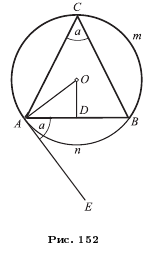
\includegraphics{mppics/ris-152}
\caption{}\label{1938/ris-152}
\end{wrapfigure}

\smallskip
\mbox{\so{Построение}.}
При конце отрезка $AB$ строим угол $DAE$, равный углу $\alpha$;
проводим срединный перпендикуляр $DO$ к $AB$ и из точки $A$ восстанавливаем перпендикуляр к $AE$; 
точку пересечения $O$ этих двух перпендикуляров принимаем за центр и радиусом $AO$ описываем окружность.

\smallskip
\mbox{\so{Доказательство}.}
Сегмент $AmB$ будет искомый, потому что всякий вписанный в него угол измеряется половиной дуги $AnB$, а половина этой дуги измеряет также $\angle DAE=\alpha$.

\smallskip
\mbox{\so{Замечание}.}
На рис.~\ref{1938/ris-152} построен сегмент, расположенный выше отрезка $AB$.
Такой же сегмент может быть построен и по другую сторону отрезка $AB$.
Таким образом, можно сказать, что геометрическое место точек, из которых данный отрезок $AB$ виден под данным углом $\alpha$, состоит из дуг двух сегментов, из которых каждый вмещает в себя угол $\alpha$ и один расположен по одну сторону отрезка $AB$, а другой — по другую сторону.

\subsection*{Задачи на построение}

\paragraph{Метод геометрических мест.}\label{1938/133}
Для решения многих задач на построение можно с успехом применять понятие о геометрическом месте и основанный на нём метод геометрических мест.
Этот метод, известный ещё со времён Платона (IV век до нашей эры), состоит в следующем.

Положим, что решение предложенной задачи сводится к нахождению некоторой точки, которая должна удовлетворять известным условиям.
Отбросим из этих условий какое-нибудь одно;
тогда задаче может удовлетворять бесчисленное множество точек.
Эти точки составят некоторое геометрическое место.
Построим его, если это окажется возможным.
Затем примем во внимание отброшенное нами условие и откинем какое-нибудь другое;
тогда задача будет снова удовлетворяться бесчисленным множеством точек, которые составят новое геометрическое место.
Построим его, если это возможно.
Искомая точка, удовлетворяя всем условиям, должна лежать на обоих геометрических местах, то есть она должна находиться в их пересечении.
Задача не имеет решения если найденные геометрические места не пересекаются;
и задача будет иметь столько решений, сколько окажется точек пересечения.

Приведём на этот метод один пример, который вместе с тем покажет нам, как иногда приходится вводить в чертёж вспомогательные линии с целью принять во внимание все данные условия задачи.

\paragraph{}\label{1938/134}
\so{Задача}.
\emph{Построить треугольник по основанию $a$, углу при вершине $A$ и сумме $s$ боковых сторон.}

\begin{wrapfigure}{o}{53mm}
\centering
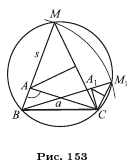
\includegraphics{mppics/ris-153}
\caption{}\label{1938/ris-153}
\end{wrapfigure}

Пусть $ABC$ будет искомый треугольник (рис.~\ref{1938/ris-153}).
Чтобы принять во внимание данную сумму боковых сторон, продолжим $BA$ и отложим $BM=s$.
Проведя $MC$, получим вспомогательный треугольник $BMC$.
Если мы построим этот треугольник, то затем легко построить искомый треугольник $ABC$.

Построение треугольника $BMC$ сводится к нахождению точки~$M$.

Заметив, что треугольник $AMC$ равнобедренный ($AM=AC$) и, следовательно, $\angle M \z=  \tfrac12\angle BAC$ (так как $\angle M+\angle MCA = \angle BAC$), мы видим, что точка $M$ должна удовлетворять двум условиям:
1) она удалена от $B$ на расстояние $s$, 
2) из неё данный отрезок $BC$ виден под углом, равным $\tfrac12\angle A$.
Отбросив второе условие, мы получим бесчисленное множество точек $M$, лежащих на окружности, описанной радиусом, равным $s$, с центром в точке $B$.
Отбросив первое условие, мы получим также бесчисленное множество точек $M$, лежащих на дуге сегмента, построенного на $BC$ и вмещающего угол, равный $\tfrac12\angle A$.
Таким образом, нахождение точки $M$ сводится к построению двух геометрических мест, из которых каждое мы построить умеем.
Задача не будет иметь решения, если эти геометрические места не будут иметь общих точек;
задача будет иметь одно или два решения, смотря по тому, касаются или же пересекаются эти геометрические места (на нашем чертеже получаются два треугольника $ABC$ и $A_1BC$, удовлетворяющие условиям задачи).

\medskip

Иногда задача сводится не к определению точки, а к нахождению прямой, удовлетворяющей нескольким условиям.
Если отбросим одно из условий, то получим бесчисленное множество прямых;
при этом может случиться, что эти прямые определяют некоторую линию (например, все они будут касательными к некоторой окружности).
Отбросив другое условие и приняв во внимание то, которое было откинуто ранее, мы получим снова бесчисленное множество прямых, которые, быть может, определят некоторую другую линию.
Построив, если возможно, эти две линии, мы затем легко найдём и искомую прямую.
Приведём пример.

\paragraph{}\label{1938/135}
\so{Задача}.
\emph{Провести секущую к двум данным окружностям с центрами $O$ и $O_1$ так, чтобы части секущей, заключённые внутри окружностей, равнялись соответственно данным отрезкам $a$ и~$a_1$.}

\begin{wrapfigure}{o}{53mm}
\vskip-2mm
\centering
\includegraphics{mppics/ris-extra-6}
\caption{}\label{extra/ris-6}
\end{wrapfigure}

Если возьмём только одно условие, например, чтобы часть секущей, лежащая внутри круга  с центром $O$, равнялась $a$, то получим бесчисленное множество секущих, которые все должны быть одинаково удалены от $O$ (так как равные хорды одинаково удалены от центра).

Поэтому, если в этом круге где-нибудь построим хорду, равную $a$, а затем радиусом, равным расстоянию от этой хорды до центра, опишем окружность, с центром в $O$, то все секущие, о которых идёт речь, должны касаться этой вспомогательной окружности.

Подобным образом, приняв во внимание только второе условие, мы увидим, что искомая секущая должна касаться второй вспомогательной окружности с центом $O_1$.
Значит, вопрос сводится к построению общей касательной к двум окружностям.

\subsection*{Упражнения}

\begin{center}
\so{Найти геометрические места}
\end{center}

\begin{enumerate}

\item
Точек, из которых касательные, проведённые к данной окружности, равны данному отрезку.
 
\item

Точек, из которых данная окружность видна под данным углом (то есть две касательные, проведённые из данной точки к окружности, составляют между собой данный угол).



\item
Центров окружностей, описанных данным радиусом и касающихся данной прямой.

\item
Центров окружностей, описанных данным радиусом и касающихся данной окружности (два случая:
касание внешнее и касание внутреннее).

\item
Отрезок данной длины движется параллельно самому себе так, что один его конец скользит по окружности.
Найти геометрическое место, описанное другим концом.

\smallskip
\so{Указание}.
Возьмём две прямые, изображающие два положения, движущейся прямой, и через концы их, лежащие на окружности, проведём радиусы, а через другие концы проведём прямые, параллельные этим радиусам, до пересечения с прямой, проходящей через центр и параллельной движущейся линии.
Рассмотрим образовавшиеся параллелограммы.

\item
Отрезок данной длины движется так, что концы его скользят по сторонам прямого угла.
Найти геометрическое место, описываемое серединой этого отрезка.

\end{enumerate}

\begin{center}
\so{Доказать теоремы}
\end{center}

\begin{enumerate}[resume]


\item
Из всех хорд, проходящих через точку $A$, взятую внутри данного круга, наименьшей будет та, которая перпендикулярна к диаметру, проходящему через точку $A$.

\item
На хорде $AB$ взяты две точки $D$ и $E$ на равном расстоянии от середины $C$ этой хорды, и через эти точки восстановлены к $AB$ перпендикуляры $DF$ и $EG$ до пересечения с окружностью.
Доказать, что эти перпендикуляры равны.

\smallskip
\so{Указание}.
Перегнуть чертёж по диаметру.

\item
В круге проведены две хорды $CC'$ и $DD'$ перпендикулярно к диаметру $AB$.
Доказать, что прямая $MM'$, соединяющая середины хорд $CD$ и $C'D'$, перпендикулярна к $AB$.

\item
В круге с центром $O$ проведена хорда $AB$ и продолжена на расстояние $BC$, равное радиусу.
Через точку $C$ и центр $O$ проведена секущая $CD$ ($D$ — вторая точка пересечения с окружностью).
Доказать, что угол $AOD$ равен утроенному углу $ACD$.

\item
Если через центр окружности и данную точку вне её проведём секущую, то часть её, заключённая между данной точкой и ближайшей точкой пересечения, есть наименьшее расстояние, а часть, заключённая между данной точкой и другой точкой пересечения, есть наибольшее расстояние от данной точки до точек окружности.

\item
Кратчайшее расстояние между двумя окружностями, лежащими одна вне другой, есть отрезок линии центров, заключённый между окружностями.

\item
Если через точку пересечения двух окружностей будем проводить секущие, не продолжая их за окружности, то наибольшей из них окажется та, которая параллельна линии центров.

\item
Если к двум окружностям, касающимся извне, провести три общие касательные, то внутренняя из них делит пополам тот отрезок каждой внешней, который ограничен точками касания.

\item
Через точку $A$ окружности проведена хорда $AB$ и затем касательная в точке $B$.
Диаметр, перпендикулярный радиусу $OA$, встречает касательную и хорду (или её продолжение) соответственно в точках $C$ и $O$.
Доказать, что $BC=CD$.

\item
К двум окружностям с центрами $O$ и $O_1$, касающимся извне в точке $A$, проведена общая внешняя касательная $BC$ ($B$ и $C$ — точки касания);
доказать, что угол $BAC$ есть прямой.

\smallskip
\so{Указание}.
Провести в точке $A$ общую касательную и рассмотреть равнобедренные треугольники $ABD$ и $ADC$.

\item
Две прямые исходят из одной и той же точки $M$ и касаются окружности в точках $A$ и $B$.
Проведя радиус $OB$, продолжают его за точку $B$ на расстояние $BC=OB$.
Доказать, что $\angle AMC\z=3\angle BMC$.

\item
Две прямые, исходящие из точки $M$, касаются окружности в точках $A$ и $B$.
На меньшей из двух дуг, ограниченных точками $A$ и $B$, берут произвольную точку $C$ и через неё проводят третью касательную до пересечения с $MA$ и $MB$ в точках $D$ и $E$.
Доказать, что:
1) периметр $\triangle MDE$ и 2) угол $DOE$ не изменяются при изменении положения точки $C$.

\smallskip
\so{Указание}.
Периметр $DME=MA+MB$, $\angle DOE\z=\tfrac12 \angle AOB$.
\end{enumerate}

%\clearpage%

\begin{center}
\so{Задачи на построение}
\end{center}

\begin{enumerate}[resume]
\item
Разделить данную дугу на $4, 8, 16, \dots$
равных частей.

\item
По сумме и разности дуг одного и того же радиуса найти эти дуги.

\item
Описать такую окружность с центром в данной точке, которая разделила бы данную окружность пополам.

\item
На данной прямой найти точку, наименее удалённую от данной окружности.

\item
В круге дана хорда.
Провести другую хорду, которая делилась бы первой пополам и составляла бы с ней данный угол (при всяком ли данном угле задача имеет решение?).

\item
Через данную в круге точку провести хорду, которая делилась бы этой точкой пополам.

\item
С центом точки на стороне данного угла, описать окружность, которая от другой стороны угла отсекла бы хорду данной длины.

\item
Данным радиусом описать окружность, центр которой лежал бы на стороне данного угла и которая от другой стороны его отсекла бы хорду данной длины.

\item
Данным радиусом описать окружность, которая касалась бы данной прямой в данной точке.

\item
Провести касательную к данной окружности параллельно данной прямой.

\item
Описать окружность, которая проходила бы через данную точку $A$ и касалась бы данной прямой в данной на ней точке $B$.

\item
Описать окружность, касательную к сторонам данного угла, причём к одной из них в данной точке.

\item
Между двумя параллельными прямыми дана точка;
провести окружность, проходящую через эту точку и касающуюся данных прямых.

\item
Провести к данной окружности касательную под данным углом к данной прямой (сколько решений?).

\item
Из точки, данной вне круга, провести к нему секущую так, чтобы её внутренняя часть равнялась данному отрезку (исследовать задачу).

\item
Данным радиусом описать окружность, проходящую через данную точку и касательную к данной прямой.

\item
На данной прямой найти такую точку, чтобы касательные, проведённые из неё к данной окружности, были данной длины.

\item
Построить треугольник, зная один угол и две высоты, из которых одна проведена из вершины данного угла.

\item
Даны две точки;
провести прямую так, чтобы перпендикуляры, опущенные на неё из этих точек, имели данные длины.

\item
Описать окружность, которая проходила бы через данную точку и касалась бы данной окружности в данной точке.

\item
Описать окружность, которая касалась бы двух данных параллельных прямых и круга, находящегося между ними.

\item
Данным радиусом описать окружность, которая касалась бы данного круга и проходила бы через данную точку.
(Рассмотреть три случая:
данная точка лежит 
1) вне круга, 
2) на окружности 
и 3) внутри круга.)

\item
Данным радиусом описать окружность, которая касалась бы данной прямой и данного круга.

\item
Данным радиусом описать окружность, которая от сторон данного угла отсекала бы хорды данной длины.

\item
Описать окружность, касающуюся данного круга в данной точке и данной прямой (два решения).

\item
Описать окружность, касающуюся данной прямой в данной точке и данного круга (два решения).

\item
Описать окружность, касающуюся двух данных кругов, причём одного из них в данной точке.
(Рассмотреть три случая:
1) искомый круг лежит вне данных кругов;
2) один из данных кругов лежит вне искомого, другой внутри;
3) оба данных круга лежат внутри искомого.)

\item
Описать окружность, касающуюся трёх равных кругов извне или внутри.

\item
В данный сектор вписать окружность, касающуюся радиусов, ограничивающих сектор, и дуги сектора.

\item
Вписать в данный круг три равных круга, которые касались бы попарно между собой и данного круга.

\item
Через точку, данную внутри круга, провести хорду так, чтобы разность её отрезков равнялась данному отрезку.

\smallskip
\so{Указание}.
Провести окружность, концентрическую данной и проходящую через данную точку.
В этой окружности от данной точки построить хорду данной длины.


\item
Через точку пересечения двух окружностей провести секущую так, чтобы часть её, заключённая внутри окружностей, равнялась данной длине.

\smallskip
\so{Указание}.
Построить прямоугольный треугольник, имеющий гипотенузой отрезок прямой, соединяющий центры данных окружностей с катетом, равным половине данного отрезка, и~т.~д.

\item
Из точки, данной вне круга, провести секущую так, чтобы внешняя часть её равнялась внутренней.

\smallskip
\so{Указание}.
Пусть $O$ — центр окружности, $R$ — её радиус, $A$~— данная точка.
Строим $\triangle AOB$, где $AB=R$, $OB=2R$.
Если $C$ — середина отрезка $OB$, то прямая $AC$ — искомая.

\item
Построить окружность касающуюся данной прямой в данной точке, и проходящую через другую данную точку.

\item
Построить окружность касающуюся двух прямых, если дана одна из точек касания.

\end{enumerate}
